\subsection{Configurazione del build.gradle}
\label{buildGradle}
Come in Maven ci sono i goals, in Gradle ci sono i tasks ognuno dei quali ha il suo scopo definito nella sua implementazione. L'implementazione dei tasks viene fatta in un file di configurazione solitamente nominato build.gradle, che non è altro che uno script in linguaggio Groovy. Creaiamo quindi una cartella in cui inserire la nostra configurazione di gradle e creiamo il file build.gradle in cui andremo a inserire:
\begin{lstlisting}[frame=single]
description = 'Example of Task'

task dependenceZero {
	description = 'Build Dependence Zero'
	doFirst {
		println 'First Zero'
	}
	doLast {
		println 'Last Zero'
	}
}

task dependenceOne(dependsOn: [dependenceZero]) {
	description = 'Build Dependence One'
	doFirst {
		println 'First One'
	}
	doLast {
		println 'Last One'
	}
}

task dependenceTwo {
	description = 'Build Dependence Two'
	doFirst {
		println 'First Two'
	}
	doLast {
		println 'Last Two'
	}
}

task mainTask(dependsOn: [dependenceOne, dependenceTwo]) {
	description = 'Build Main Task'
	doFirst {
		println 'First MainTask'
	}
	doLast {
		println 'Last MainTask'
	}
}
\end{lstlisting}
In questa build abbiamo definito 4 task: dependenceZero, dependeceOne, dependenceTwo e mainTask. Nella definizione del task può essere usata la parola \textsc{dependsOn} per indicare che il task definito dipende da uno o più task. Nel caso di dependenceOne abbiamo una sola dipendenza che è dependenceZero, nel caso invece di taskMain si hanno 2 dipendenze che sono dependenceOne e dependenceTwo. Possiamo notare che si è data una descrizione sia dei tasks che della build, questo non serve nella pratica ma è buona norma dare sempre una spiegazione sia della build che dei nuovi task che si creano. All'interno dei tasks si nota che ci sono definite delle azioni: doFirst e doLast, quando sarà eseguita la build di un task verrà eseguita prima doFirst e infine doLast. Con la configurazione precedente abbiamo creato un albero delle dipendenze di questo tipo:
\begin{figure}[H]
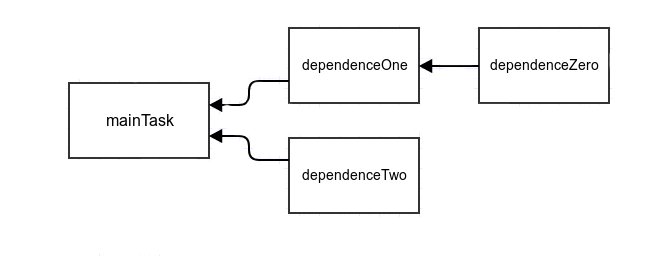
\includegraphics[scale=0.40]{1Task/task_taskDep/graphDep.png}
\end{figure}
Le builds di gradle vengono eseguite usando il comando da terminale \texttt{\$ gradle taskName}, per l'esempio è possibile quindi eseguire le builds:
\begin{itemize}
    \item \begin{verbatim} $ gradle dependenceZero \end{verbatim}
    \item \begin{verbatim} $ gradle dependenceOne \end{verbatim}
    \item \begin{verbatim} $ gradle dependenceTwo \end{verbatim}
    \item \begin{verbatim} $ gradle mainTask \end{verbatim}
\end{itemize}
Ma è anche possibile eseguire più task contemporaneamente, per esempio:
\begin{itemize}
    \item \begin{verbatim} $ gradle dependenceZero mainTask\end{verbatim}
    \item \begin{verbatim} $ gradle dependenceOne dependenceTwo \end{verbatim}
    \item \begin{verbatim} $ gradle dependenceOne dependenceTwo mainTask\end{verbatim}
\end{itemize}
Considerando che il mainTask è dipendente da dependenceOne e dependenceTwo, l'ultimo esempio non aggiunge niente di più alla build dato che verrebbero comunque eseguiti i 2 tasks. Se eseguiamo infatti
\begin{verbatim}
    $ gradle mainTask \end{verbatim} 
e poi 
\begin{verbatim}
    $ gradle dependenceOne dependenceTwo mainTask \end{verbatim}
otterremo il solito output, che è il seguende:
\label{outMainTask}
\begin{verbatim}
> Task :dependenceZero 
First Zero
Last Zero
> Task :dependenceOne 
First One
Last One
> Task :dependenceTwo 
First Two
Last Two
> Task :mainTask 
First MainTask
Last MainTask
BUILD SUCCESSFUL in 0s
4 actionable tasks: 4 executed\end{verbatim} 
